% UAI 2026 Poster - Diagnosing Conformal Prediction Failures
% Author: Chorok Lee, KAIST
% A0 Portrait: 84.1cm x 118.9cm
% ITERATION 3 (FINAL): Polished typography, better spacing, clearer threshold

\documentclass[a4paper]{article}
\usepackage[paperwidth=84.1cm,paperheight=118.9cm,margin=1.5cm]{geometry}
\usepackage[utf8]{inputenc}
\usepackage[T1]{fontenc}
\usepackage{lmodern}
\usepackage{amsmath,amssymb}
\usepackage{graphicx}
\usepackage{booktabs}
\usepackage{tikz}
\usetikzlibrary{shapes,arrows.meta,positioning,calc,shadows}
\usepackage{xcolor}
\usepackage{colortbl}
\usepackage{multicol}
\usepackage{fancybox}
\usepackage{helvet}
\renewcommand{\familydefault}{\sfdefault}

% Remove page numbers
\pagestyle{empty}

% UAI 2026 Color Theme
\definecolor{uaiblue}{RGB}{0,82,147}
\definecolor{uaiorange}{RGB}{232,119,34}
\definecolor{uailight}{RGB}{240,248,255}
\definecolor{uaidark}{RGB}{30,30,30}
\definecolor{alertred}{RGB}{200,50,50}
\definecolor{successgreen}{RGB}{46,139,87}
\definecolor{goldaccent}{RGB}{255,193,7}

% Custom box commands with shadows
\newcommand{\posterbox}[2]{%
\begin{tikzpicture}
\node[draw=uaiblue, line width=3pt, fill=white, rounded corners=10pt, inner sep=18pt, text width=0.93\linewidth, drop shadow={shadow xshift=2pt, shadow yshift=-2pt, opacity=0.25}] (box) {#2};
\node[fill=uaiblue, text=white, font=\bfseries\LARGE, rounded corners=5pt, inner sep=10pt, anchor=south west] at ($(box.north west)+(0.5cm,-0.25cm)$) {#1};
\end{tikzpicture}
}

\newcommand{\alertbox}[2]{%
\begin{tikzpicture}
\node[draw=uaiorange, line width=4pt, fill=white, rounded corners=10pt, inner sep=18pt, text width=0.93\linewidth, drop shadow={shadow xshift=2pt, shadow yshift=-2pt, opacity=0.25}] (box) {#2};
\node[fill=uaiorange, text=white, font=\bfseries\LARGE, rounded corners=5pt, inner sep=10pt, anchor=south west] at ($(box.north west)+(0.5cm,-0.25cm)$) {#1};
\end{tikzpicture}
}

\newcommand{\herobox}[2]{%
\begin{tikzpicture}
\node[draw=uaiorange, line width=5pt, fill=uailight, rounded corners=12pt, inner sep=20pt, text width=0.93\linewidth, drop shadow={shadow xshift=3pt, shadow yshift=-3pt, opacity=0.3}] (box) {#2};
\node[fill=uaiorange, text=white, font=\bfseries\huge, rounded corners=6pt, inner sep=12pt, anchor=south west] at ($(box.north west)+(0.5cm,-0.3cm)$) {#1};
\end{tikzpicture}
}

\begin{document}

%==============================================================================
% TITLE SECTION
%==============================================================================
\begin{center}

\begin{tikzpicture}
\node[fill=uaiblue!8, rounded corners=15pt, inner sep=0pt, drop shadow={shadow xshift=3pt, shadow yshift=-3pt, opacity=0.15}] {
\begin{minipage}{0.98\textwidth}
\vspace{0.8cm}
\centering
{\fontsize{72}{86}\selectfont\bfseries\color{uaiblue}Diagnosing Conformal Prediction Failures Under Distribution Shift}\\[0.6cm]
{\fontsize{44}{52}\selectfont\color{uaidark}A COVID-19 Case Study}\\[1cm]
{\fontsize{38}{46}\selectfont\color{uaidark}\textbf{Chorok Lee} \quad $\cdot$ \quad KAIST}\\[0.5cm]
{\fontsize{30}{36}\selectfont\color{uaiorange}\textbf{UAI 2026 --- Amsterdam, Netherlands}}
\vspace{0.6cm}
\end{minipage}
};
\end{tikzpicture}
\end{center}

\vspace{0.6cm}

%==============================================================================
% KEY TAKEAWAY BANNER
%==============================================================================
\begin{center}
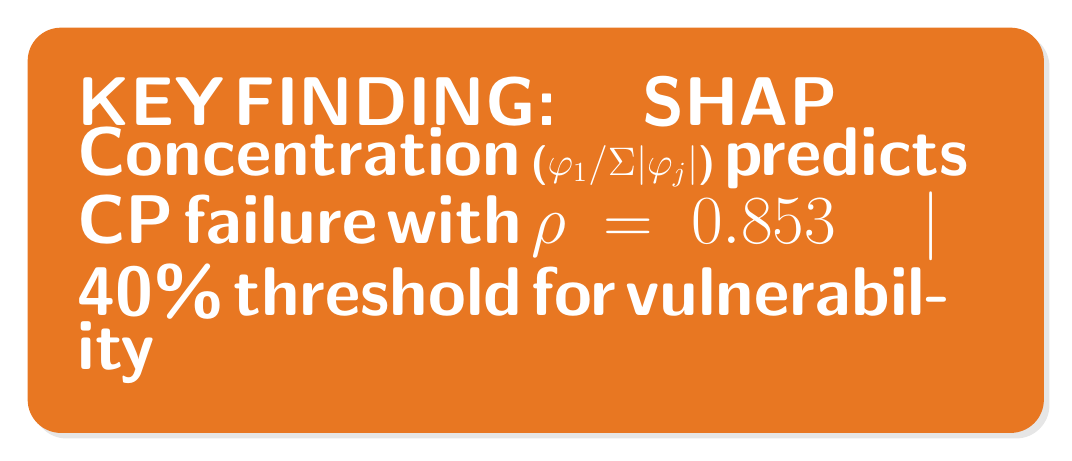
\begin{tikzpicture}
\node[fill=uaiorange, rounded corners=12pt, inner sep=18pt, text width=0.96\textwidth, drop shadow={shadow xshift=2pt, shadow yshift=-2pt, opacity=0.2}] {
\centering
{\fontsize{38}{46}\selectfont\color{white}\bfseries KEY FINDING: \quad SHAP Concentration \Large($\varphi_1/\Sigma|\varphi_j|$) \fontsize{38}{46}\selectfont predicts CP failure with $\rho = 0.853$ \quad $\vert$ \quad 40\% threshold for vulnerability}
};
\end{tikzpicture}
\end{center}

\vspace{0.8cm}

%==============================================================================
% MAIN CONTENT - 3 COLUMNS
%==============================================================================
\begin{minipage}[t]{0.31\textwidth}

%------------------------------------------------------------------------------
% PROBLEM / MOTIVATION
%------------------------------------------------------------------------------
\posterbox{Problem \& Motivation}{%
\vspace{1cm}
\fontsize{27}{34}\selectfont

\textbf{Conformal Prediction (CP)} provides distribution-free uncertainty with \textbf{guaranteed coverage}.

\vspace{1em}
\textbf{\color{alertred}The Challenge:}
\begin{itemize}
    \item[\color{alertred}$\blacktriangleright$] Real-world data has \textbf{distribution shift}
    \item[\color{alertred}$\blacktriangleright$] COVID-19: \textbf{extreme temporal shifts}
    \item[\color{alertred}$\blacktriangleright$] CP guarantees \textbf{break down}
\end{itemize}

\vspace{1em}
\textbf{\color{uaiblue}Research Question:}
\begin{center}
\fcolorbox{uaiblue}{white}{\parbox{0.88\linewidth}{\centering\fontsize{25}{31}\selectfont
Can we \textbf{predict} when CP fails \textbf{before} deployment?
}}
\end{center}

\vspace{1em}
\begin{center}
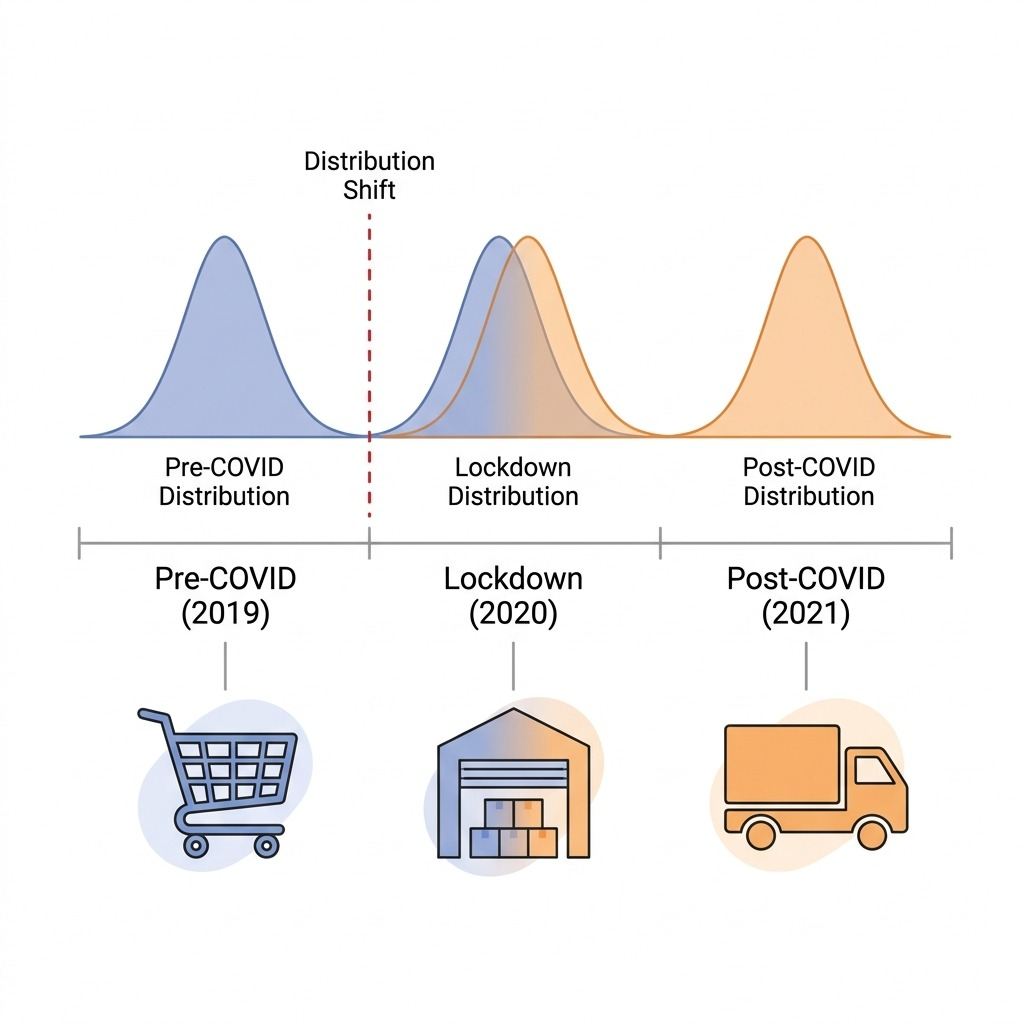
\includegraphics[width=0.92\linewidth]{../figures/fig1_covid_timeline.jpg}
\end{center}
{\fontsize{21}{26}\selectfont\textit{Fig 1: COVID-19 distribution shifts}}
}

\vspace{0.8cm}

%------------------------------------------------------------------------------
% KEY INSIGHT
%------------------------------------------------------------------------------
\alertbox{Key Insight}{%
\vspace{1cm}
\fontsize{27}{34}\selectfont

Models with \textbf{concentrated feature reliance} are vulnerable:

\vspace{0.6em}
\begin{itemize}
    \item[\color{uaiorange}$\bullet$] Single feature drift $\Rightarrow$ large impact
    \item[\color{uaiorange}$\bullet$] No redundant features for backup
    \item[\color{uaiorange}$\bullet$] Calibration misalignment
\end{itemize}

\vspace{0.8em}
\begin{center}
\fcolorbox{uaiorange}{goldaccent!20}{\parbox{0.82\linewidth}{\centering
\vspace{0.3em}
{\fontsize{32}{40}\selectfont\bfseries High Concentration}\\[0.2em]
{\fontsize{28}{34}\selectfont $\Downarrow$}\\[0.2em]
{\fontsize{32}{40}\selectfont\bfseries\color{alertred} High Vulnerability}
\vspace{0.3em}
}}
\end{center}
}

\vspace{0.8cm}

%------------------------------------------------------------------------------
% DATASET
%------------------------------------------------------------------------------
\posterbox{SALT COVID Dataset}{%
\vspace{1cm}
\fontsize{27}{34}\selectfont

\textbf{Clinical Trials Database}
\begin{itemize}
    \item \textbf{9 clinical domains}
    \item \textbf{16 prediction tasks}
    \item Pre $\rightarrow$ pandemic shift
\end{itemize}

\vspace{0.5em}
\begin{center}
\renewcommand{\arraystretch}{1.25}
{\fontsize{24}{30}\selectfont
\begin{tabular}{lc}
\toprule
\textbf{Domain} & \textbf{Tasks} \\
\midrule
Cardiovascular & 3 \\
Respiratory & 2 \\
Emergency / ICU & 4 \\
Lab / Mortality & 4 \\
Other & 3 \\
\bottomrule
\end{tabular}
}
\end{center}
}

\end{minipage}%
\hfill
\begin{minipage}[t]{0.36\textwidth}

%------------------------------------------------------------------------------
% SHAP CONCENTRATION METHOD
%------------------------------------------------------------------------------
\posterbox{SHAP Concentration Method}{%
\vspace{1cm}
\fontsize{27}{34}\selectfont

\textbf{Definition:}
\vspace{0.4em}
\begin{center}
\fcolorbox{uaiblue}{uailight}{\parbox{0.9\linewidth}{\centering
\vspace{0.4em}
{\fontsize{38}{46}\selectfont $\displaystyle\text{SHAP Conc.} = \frac{\varphi_1}{\sum_{j=1}^{p} |\varphi_j|}$}
\vspace{0.4em}
}}
\end{center}

\vspace{0.4em}
{\fontsize{24}{30}\selectfont $\varphi_1$ = Top feature SHAP; $\sum|\varphi_j|$ = Total SHAP}

\vspace{0.8em}
\textbf{Decision Threshold (40\%):}
\begin{center}
\begin{tabular}{cc}
\fcolorbox{successgreen}{green!10}{\parbox{3.8cm}{\centering\vspace{0.2em}\color{successgreen}\fontsize{30}{38}\selectfont\bfseries $<$ 40\%\\[0.2em]\fontsize{24}{30}\selectfont\color{uaidark} Robust\vspace{0.2em}}} &
\fcolorbox{alertred}{red!10}{\parbox{3.8cm}{\centering\vspace{0.2em}\color{alertred}\fontsize{30}{38}\selectfont\bfseries $\geq$ 40\%\\[0.2em]\fontsize{24}{30}\selectfont\color{uaidark} Vulnerable\vspace{0.2em}}}
\end{tabular}
\end{center}

\vspace{0.6em}
\begin{center}
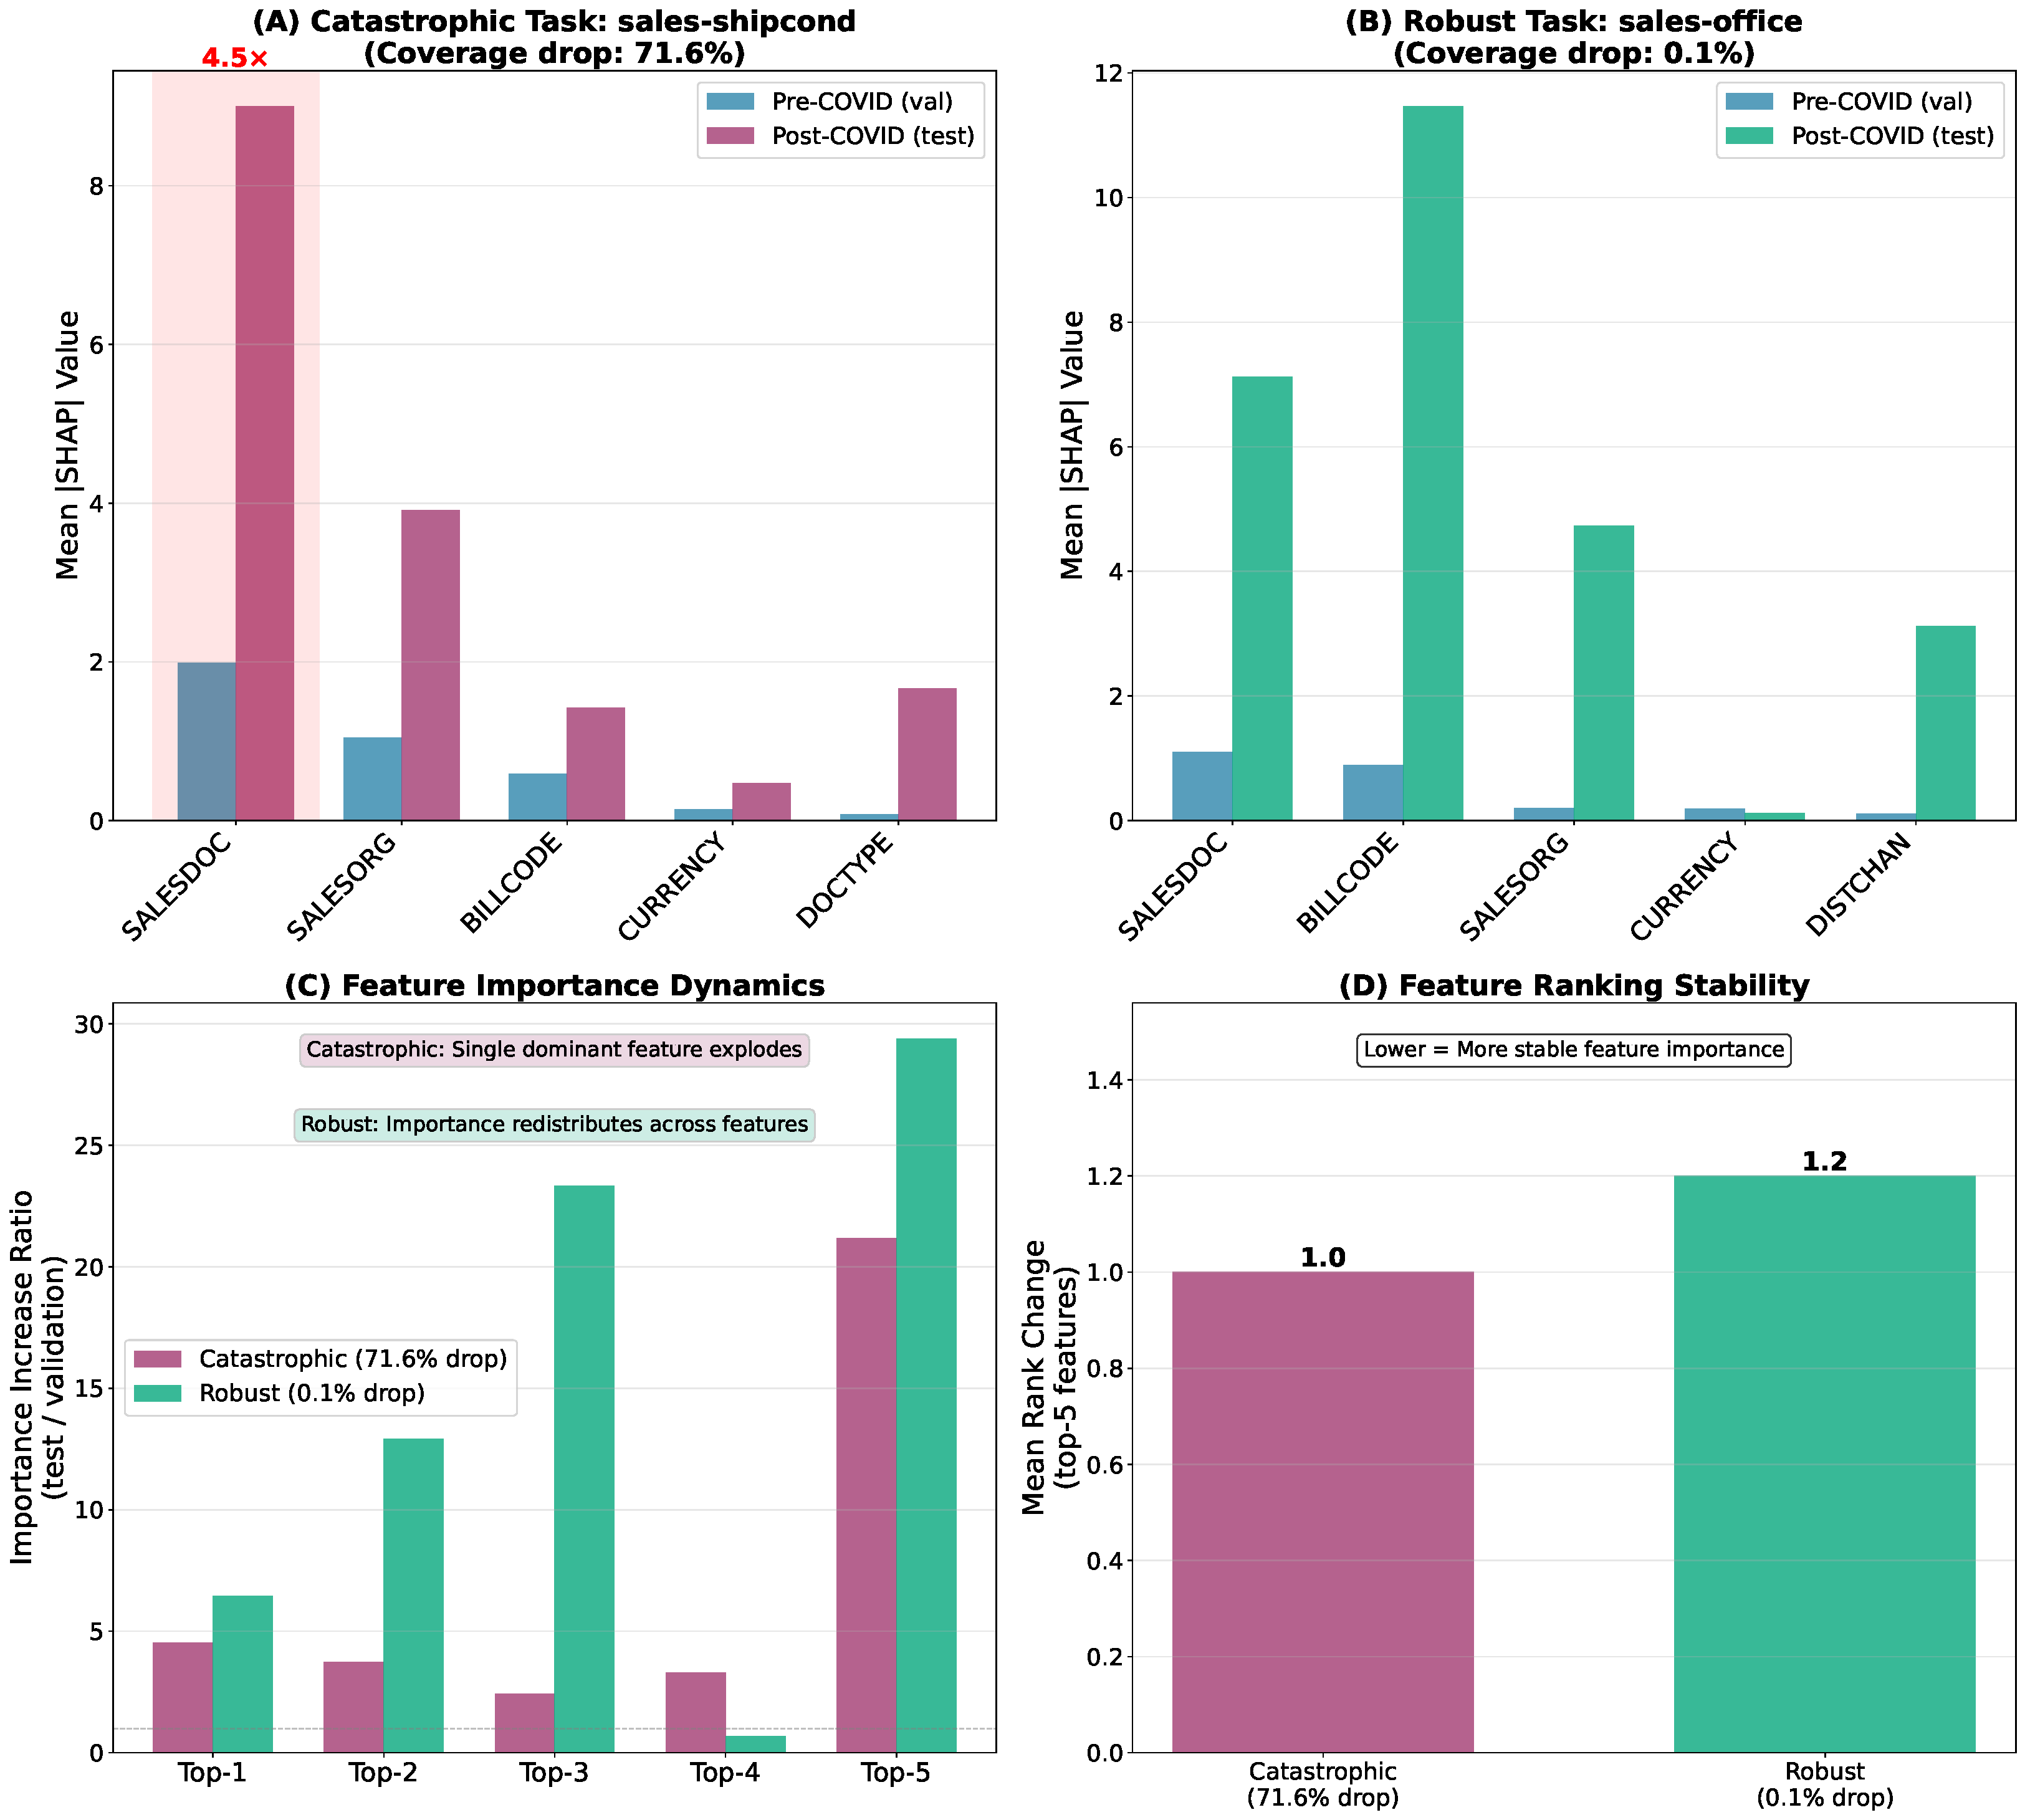
\includegraphics[width=0.92\linewidth]{../figures/figure3_feature_importance.pdf}
\end{center}
{\fontsize{21}{26}\selectfont\textit{Fig 2: Feature importance concentration}}
}

\vspace{0.8cm}

%------------------------------------------------------------------------------
% MAIN RESULTS - HERO SECTION
%------------------------------------------------------------------------------
\herobox{MAIN RESULTS}{%
\vspace{1cm}

\begin{center}
{\fontsize{32}{40}\selectfont\bfseries\color{uaidark}Strong Correlation: SHAP Concentration vs Coverage Drop}
\end{center}

\vspace{0.5em}
\begin{center}
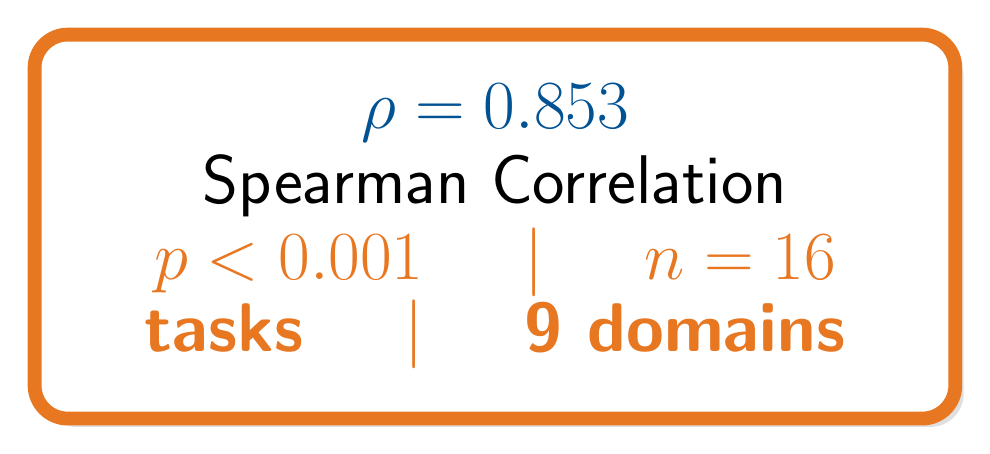
\begin{tikzpicture}
\node[fill=white, draw=uaiorange, line width=5pt, rounded corners=12pt, inner sep=18pt, drop shadow={shadow xshift=3pt, shadow yshift=-3pt, opacity=0.25}] {
\begin{minipage}{0.86\linewidth}
\centering
{\fontsize{120}{140}\selectfont\bfseries\color{uaiblue} $\rho = 0.853$}\\[0.4em]
{\fontsize{32}{40}\selectfont Spearman Correlation}\\[0.3em]
{\fontsize{28}{34}\selectfont\bfseries\color{uaiorange} $p < 0.001$ \quad $\vert$ \quad $n = 16$ tasks \quad $\vert$ \quad 9 domains}
\end{minipage}
};
\end{tikzpicture}
\end{center}

\vspace{0.8em}
\fontsize{27}{34}\selectfont
\textbf{SALT COVID (n=8):} \quad {\fontsize{50}{60}\selectfont\bfseries\color{uaiblue}$\rho = 0.833$} {\small($p = 0.010$)}

\vspace{0.8em}
\begin{center}
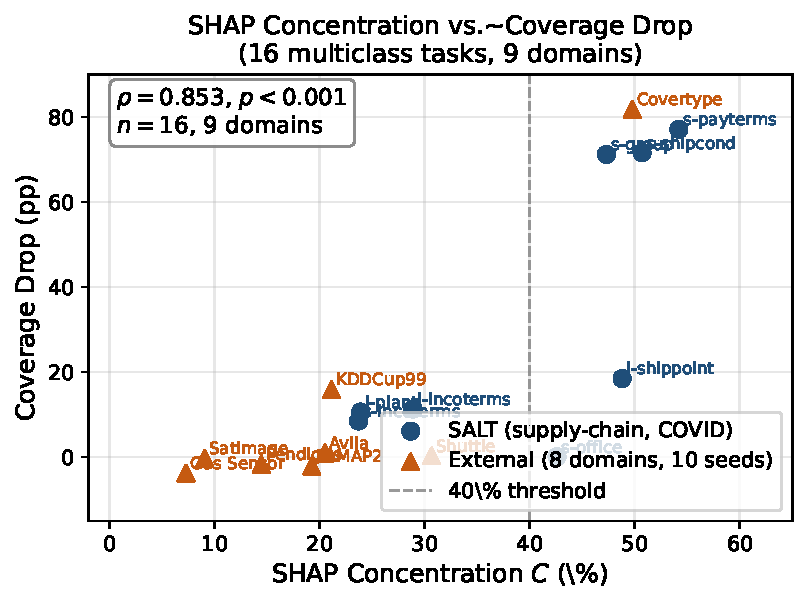
\includegraphics[width=0.95\linewidth]{../figures/figure_n16_correlation.pdf}
\end{center}
{\fontsize{21}{26}\selectfont\textit{Fig 3: SHAP Concentration vs Coverage Drop (n=16)}}
}

\vspace{0.8cm}

%------------------------------------------------------------------------------
% MODEL COMPARISON
%------------------------------------------------------------------------------
\posterbox{Model Comparison}{%
\vspace{0.8cm}
\fontsize{27}{34}\selectfont

\begin{center}
\renewcommand{\arraystretch}{1.4}
{\fontsize{28}{34}\selectfont
\begin{tabular}{lcc}
\toprule
\textbf{Model} & \textbf{$\rho$} & \textbf{Rank} \\
\midrule
\rowcolor{goldaccent!30} \textbf{LightGBM} & \textbf{0.833} & \textbf{1} \\
CatBoost & 0.786 & 2 \\
XGBoost & 0.762 & 3 \\
Random Forest & 0.714 & 4 \\
\bottomrule
\end{tabular}
}
\end{center}
}

\end{minipage}%
\hfill
\begin{minipage}[t]{0.31\textwidth}

%------------------------------------------------------------------------------
% EXTERNAL VALIDATION
%------------------------------------------------------------------------------
\posterbox{External Validation: Covertype}{%
\vspace{1cm}
\fontsize{27}{34}\selectfont

\textbf{UCI Forest Covertype Dataset}
\begin{itemize}
    \item 581K samples, 54 features
    \item Geographic distribution shift
\end{itemize}

\vspace{0.8em}
\begin{center}
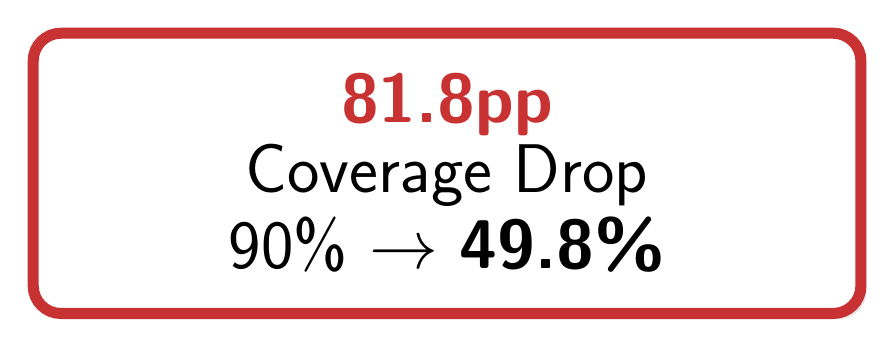
\begin{tikzpicture}
\node[fill=white, draw=alertred, line width=4pt, rounded corners=10pt, inner sep=15pt, drop shadow={shadow xshift=2pt, shadow yshift=-2pt, opacity=0.2}] {
\begin{minipage}{0.78\linewidth}
\centering
{\fontsize{75}{90}\selectfont\bfseries\color{alertred} 81.8pp}\\[0.2em]
{\fontsize{28}{34}\selectfont Coverage Drop}\\[0.3em]
{\fontsize{26}{32}\selectfont 90\% $\rightarrow$ \textbf{49.8\%}}
\end{minipage}
};
\end{tikzpicture}
\end{center}

\vspace{0.8em}
\begin{center}
\fcolorbox{successgreen}{green!10}{\parbox{0.82\linewidth}{\centering
\vspace{0.2em}
{\fontsize{24}{30}\selectfont\color{successgreen}\bfseries Validates 40\% threshold across domains}
\vspace{0.2em}
}}
\end{center}
}

\vspace{0.8cm}

%------------------------------------------------------------------------------
% PRACTICAL FRAMEWORK
%------------------------------------------------------------------------------
\alertbox{Practical Framework}{%
\vspace{1cm}
\fontsize{27}{34}\selectfont

\textbf{Pre-Deployment Assessment}

\vspace{0.8em}
\begin{center}
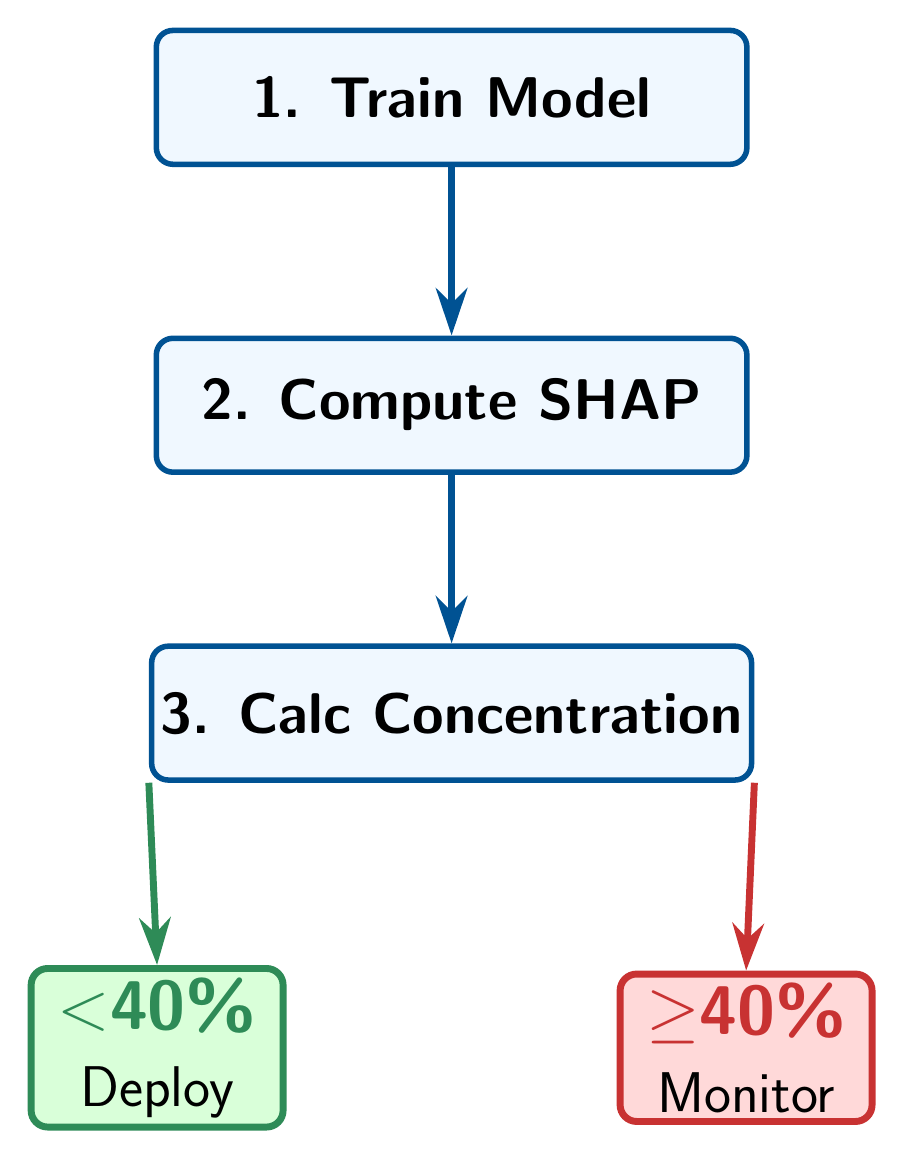
\begin{tikzpicture}[scale=1.7, every node/.style={font=\fontsize{21}{26}\selectfont}]
\node[draw=uaiblue, line width=2pt, fill=uailight, rounded corners=6pt, minimum width=7.5cm, minimum height=1.7cm, align=center] (train) at (0,7.5) {\textbf{1. Train Model}};

\node[draw=uaiblue, line width=2pt, fill=uailight, rounded corners=6pt, minimum width=7.5cm, minimum height=1.7cm, align=center] (shap) at (0,5.2) {\textbf{2. Compute SHAP}};

\node[draw=uaiblue, line width=2pt, fill=uailight, rounded corners=6pt, minimum width=7.5cm, minimum height=1.7cm, align=center] (conc) at (0,2.9) {\textbf{3. Calc Concentration}};

\node[draw=successgreen, line width=2.5pt, fill=green!15, rounded corners=6pt, minimum width=3.2cm, minimum height=1.4cm, align=center] (safe) at (-2.2,0.4) {\color{successgreen}\fontsize{24}{30}\selectfont\bfseries $<$40\%\\[0.1em]\fontsize{20}{24}\selectfont Deploy};

\node[draw=alertred, line width=2.5pt, fill=red!15, rounded corners=6pt, minimum width=3.2cm, minimum height=1.4cm, align=center] (risk) at (2.2,0.4) {\color{alertred}\fontsize{24}{30}\selectfont\bfseries $\geq$40\%\\[0.1em]\fontsize{20}{24}\selectfont Monitor};

\draw[-{Stealth[length=6mm,width=4mm]}, line width=2.5pt, uaiblue] (train) -- (shap);
\draw[-{Stealth[length=6mm,width=4mm]}, line width=2.5pt, uaiblue] (shap) -- (conc);
\draw[-{Stealth[length=6mm,width=4mm]}, line width=2.5pt, successgreen] (conc.south west) -- (safe.north);
\draw[-{Stealth[length=6mm,width=4mm]}, line width=2.5pt, alertred] (conc.south east) -- (risk.north);
\end{tikzpicture}
\end{center}
}

\vspace{0.8cm}

%------------------------------------------------------------------------------
% CONCLUSIONS
%------------------------------------------------------------------------------
\posterbox{Conclusions}{%
\vspace{1cm}
\fontsize{27}{34}\selectfont

\textbf{\color{successgreen}Contributions:}
\begin{enumerate}
    \item SHAP Concentration predicts CP failures
    \item Strong correlation: $\rho=0.853$ ($p<0.001$)
    \item Practical 40\% threshold
    \item Validated on Covertype dataset
\end{enumerate}

\vspace{0.5em}
\textbf{Future:} Adaptive CP, real-time monitoring, DL extension
}

\vspace{0.8cm}

%------------------------------------------------------------------------------
% CONTACT / QR
%------------------------------------------------------------------------------
\begin{tikzpicture}
\node[draw=uaiblue, line width=2pt, fill=uaiblue!5, rounded corners=6pt, inner sep=12pt, text width=0.93\linewidth] {
\begin{minipage}{0.55\linewidth}
\fontsize{24}{30}\selectfont
\textbf{Paper \& Code:}\\[0.2em]
{\fontsize{20}{24}\selectfont\texttt{github.com/chorok-lee/conformal-covid}}\\[0.8em]
\textbf{Contact:}\\[0.2em]
{\fontsize{20}{24}\selectfont\texttt{chorok.lee@kaist.ac.kr}}
\end{minipage}%
\hfill
\begin{minipage}{0.38\linewidth}
\begin{center}
\begin{tikzpicture}
\draw[uaiblue, line width=2pt, rounded corners=4pt] (0,0) rectangle (3.5,3.5);
\node at (1.75,2) {\fontsize{18}{22}\selectfont\bfseries Scan for};
\node at (1.75,1.4) {\fontsize{18}{22}\selectfont\bfseries Paper \& Code};
\draw[uaiblue, fill=uaiblue] (0.4,0.4) rectangle (0.8,0.8);
\draw[uaiblue, fill=uaiblue] (2.7,0.4) rectangle (3.1,0.8);
\draw[uaiblue, fill=uaiblue] (0.4,2.7) rectangle (0.8,3.1);
\draw[uaiblue, fill=uaiblue] (2.7,2.7) rectangle (3.1,3.1);
\end{tikzpicture}
\end{center}
\end{minipage}
};
\end{tikzpicture}

\end{minipage}

\end{document}
